\documentclass{beamer}
\usetheme{Madrid} 
\useinnertheme{rounded}
\usecolortheme{default}
\usepackage[orientation=landscape,size=custom,width=16,height=9,scale=0.4,debug]{beamerposter} 
\usepackage{booktabs}
\usepackage{tikz}

\title{System Identification in the frequency domain}
\author{Peter de Lange}
\institute{UC DAVIS}

\date{\today}
\begin{document}

\begin{frame}
		\titlepage
\end{frame}

\begin{frame}{System Identification}
				\begin{itemize}
				\item System Identification involves the estimation of relationships between signals.
				\item Noise is the common enemy: Introduces uncertainty in terms of variance (random errors).
				\item Learning goals;
						\begin{itemize}
						\item How to estimate relationships
						\item How to minimize uncertainty
						\end{itemize}
		\end{itemize}
\end{frame}

\begin{frame}{Systems and Models}
%Systems are expressed by signals relationships. A signal has a {domain}; time, space, frequency. And {range}; meter, Newton, Voltage, etc.\\ 
%\\
A system ${N}$ transforms input $\mathbf{u}(t)$ into output $\mathbf{y}(t)$:
		\begin{equation}
		\mathbf{y}(t) = {N}(\mathbf{u}(t))
		\end{equation}
A model ${M}$ estimates output $\mathbf{\hat{y}}(t)$ from input $\mathbf{u}(t)$ based on its model parameters $\boldsymbol{\theta}$:
		\begin{equation}
		\mathbf{\hat{y}}(t) = {M}(\boldsymbol{\theta},\mathbf{u}(t))
		\end{equation}
		\begin{itemize}
		\item Parametricmodels: few parameters, in many cases with a physical meaning.
		\item Nonparametricmodels: many parameters with no physical meaning.
		\end{itemize}
\end{frame}

\begin{frame}{Assumptions}
		The following assumptions are made for the rest of the analysis.
		\begin{itemize}
		\item	System is time invariant:
		\begin{equation}
		\mathbf{y}(t) = N(\mathbf{u}(t)) \  \rightarrow \ \mathbf{y}(t-\tau) = N(\mathbf{u}(t-\tau)) \ \ , \ \forall \tau \in R
		\end{equation}
		\item No process noise $\mathbf{w}(t)$, e.i. the system is deterministic.
		\item Observer noise $\mathbf{n}(t)$ is assumed to be Gaussian white noise.
		\end{itemize}
\end{frame}

\begin{frame}{Correlation functions}
		Correlation functions reveal structures of signals that are not apparently detectable in the time series.
		\begin{itemize}
		\item Correlation function:
				\begin{equation} \Phi_{uy}(\tau) = E\left[u(t-\tau)y(t)\right] \end{equation}
		\item Covariance function:
				\begin{equation} C_{uy}(\tau) = E\left[\left(u(t-\tau)-\mu_u\right)\left(y(t)-\mu_y\right)\right] =   \Phi_{uy}(\tau) - \mu_y\mu_y \end{equation} 
		\item Correlation coefficient:
				\begin{equation} r_{uy}(\tau) = E\left[ \left(\frac{u(t-\tau)-\mu_u}{\sigma_u}\right)\left(\frac{y(t)-\mu_y}{\sigma_y}\right)\right]  = 
				   \frac{C_{uy}(\tau)}{\sqrt{C_{uu}(0)C_{yy}(0)}} \end{equation}
		\end{itemize}
\end{frame}

\begin{frame}{Fourier transformation}
		Maps time domain signals into the frequency domain.
		\begin{itemize}
				\item Discrete Fourier transform:
				\begin{equation}
						\mathbf{u}(\omega) = \mathfrak{F}(\mathbf{u}(t)) = 2\pi\sum_{t=1}^N\mathbf{u}(t)e^{-j\omega\pi\frac{t}{N}} 
				\end{equation}
		\item Inverse discrete Fourier transform
	 				\begin{equation}
						\mathbf{u}(t) = \mathfrak{F}^{-1}(\mathbf{u}(\omega)) = \frac{1}{2\pi N} \sum_{f=1}^N\mathbf{u}(\omega)e^{j\omega\pi\frac{t}{N}} 
				\end{equation}
		\end{itemize}
\end{frame}

\begin{frame}{Spectral functions}
Next we take the Fourier transformation of the correlation functions. By doing so we obtain:
		\begin{itemize}
		\item Spectral density:
				\begin{equation}
				\hat{S}_{uy}(\omega) =  \mathfrak{F}\{\Phi_{uy}\} = \frac{1}{N}u^*(\omega)y(\omega)
				\end{equation}
		\item Coherence:
				\begin{equation}
				\hat{\gamma}^2_{uy}(\omega)  = \frac{\left|\hat{S}_{uy}(\omega)\right|^2}{\hat{S}_{uu}(\omega)\hat{S}_{yy}(\omega)}
				\end{equation}
		\end{itemize}
\end{frame}

\begin{frame}{Overview signal functions}
		The following table gives an overview of the correlatation and spectral functions and how they can be obtained:
		\begin{table}
		\begin{tabular}{lc|c|cr}
				\toprule
				\multicolumn{2}{c|}{Time domain}  & FT & \multicolumn{2}{c}{Frequency domain}  \\
				\midrule
				Input, output & $u(t)$, $y(t)$ &$\leftrightarrow$ & $u(\omega)$, $y(\omega)$ &  Input, output\\
					& $\downarrow$ &  & $\downarrow$ & \\
				Cross-correlation & $\Phi_{uy}(\tau)$ &$\leftrightarrow$  & $S_{uy}(\omega)$ & Cross-spectral density \\
					& $\downarrow$ &   &$\downarrow$  &\\
				Cross-covariance & $C_{uy}(\tau)$ & &$\downarrow$ &  \\
					& $\downarrow$ &   & $\downarrow$  &\\
				Correlation coefficient & $r_{uy}(\tau)$ & & $\gamma_{uy}(\omega)$  & Coherency  \\
				\bottomrule
		\end{tabular}
		\end{table}
\end{frame}

\begin{frame}{Experiment considerations}
\begin{itemize}
\item Measurement time $T$: Determines frequency resolution:
\begin{equation}\Delta f = \frac{1}{T}\end{equation}%: Longer measurement time increases the frequency resolution.
\item Sampling frequency $f_s$: Determines frequency bandwidth:
\begin{equation} f_n = \frac{f_s}{2} \end{equation}%: Increasing the sampling frequency increased the frequency bandwidth (Shannon's Sampling Theorem).
\item Input signal $u(t)$%: design the input signal, such that a good signal to noise ratio is achieved for a desired bandwidth.
\end{itemize}
\end{frame}

\begin{frame}{Input signal design}
Commonly used input signals for frequency domain estimation:
		\begin{table}
				\centering
				\begin{tabular}{lrrrr}
				\toprule
																					& White noise & Swept sine & Multisine & Crested  \\
				\midrule
				Mean ($\mu_u$):					& 0 & 0 & 0 & 0 \\
				Correlation ($R_{uu}$):	& 1 & 1 & 1 & 1 \\
				Spectral density ($S_{uu}):$ 										& 1.0145 &   2.4912  &  2.5000  &  2.5000 \\
				Crest factor ($C$): 						& 3.6129   & 1.4026  &  3.2857   & 2.3943 \\
				Predictable: 								& no & yes & no & no \\
				\bottomrule
				\end{tabular}
		\end{table}
\end{frame}

\begin{frame}{Input signal design}
		\begin{figure}
		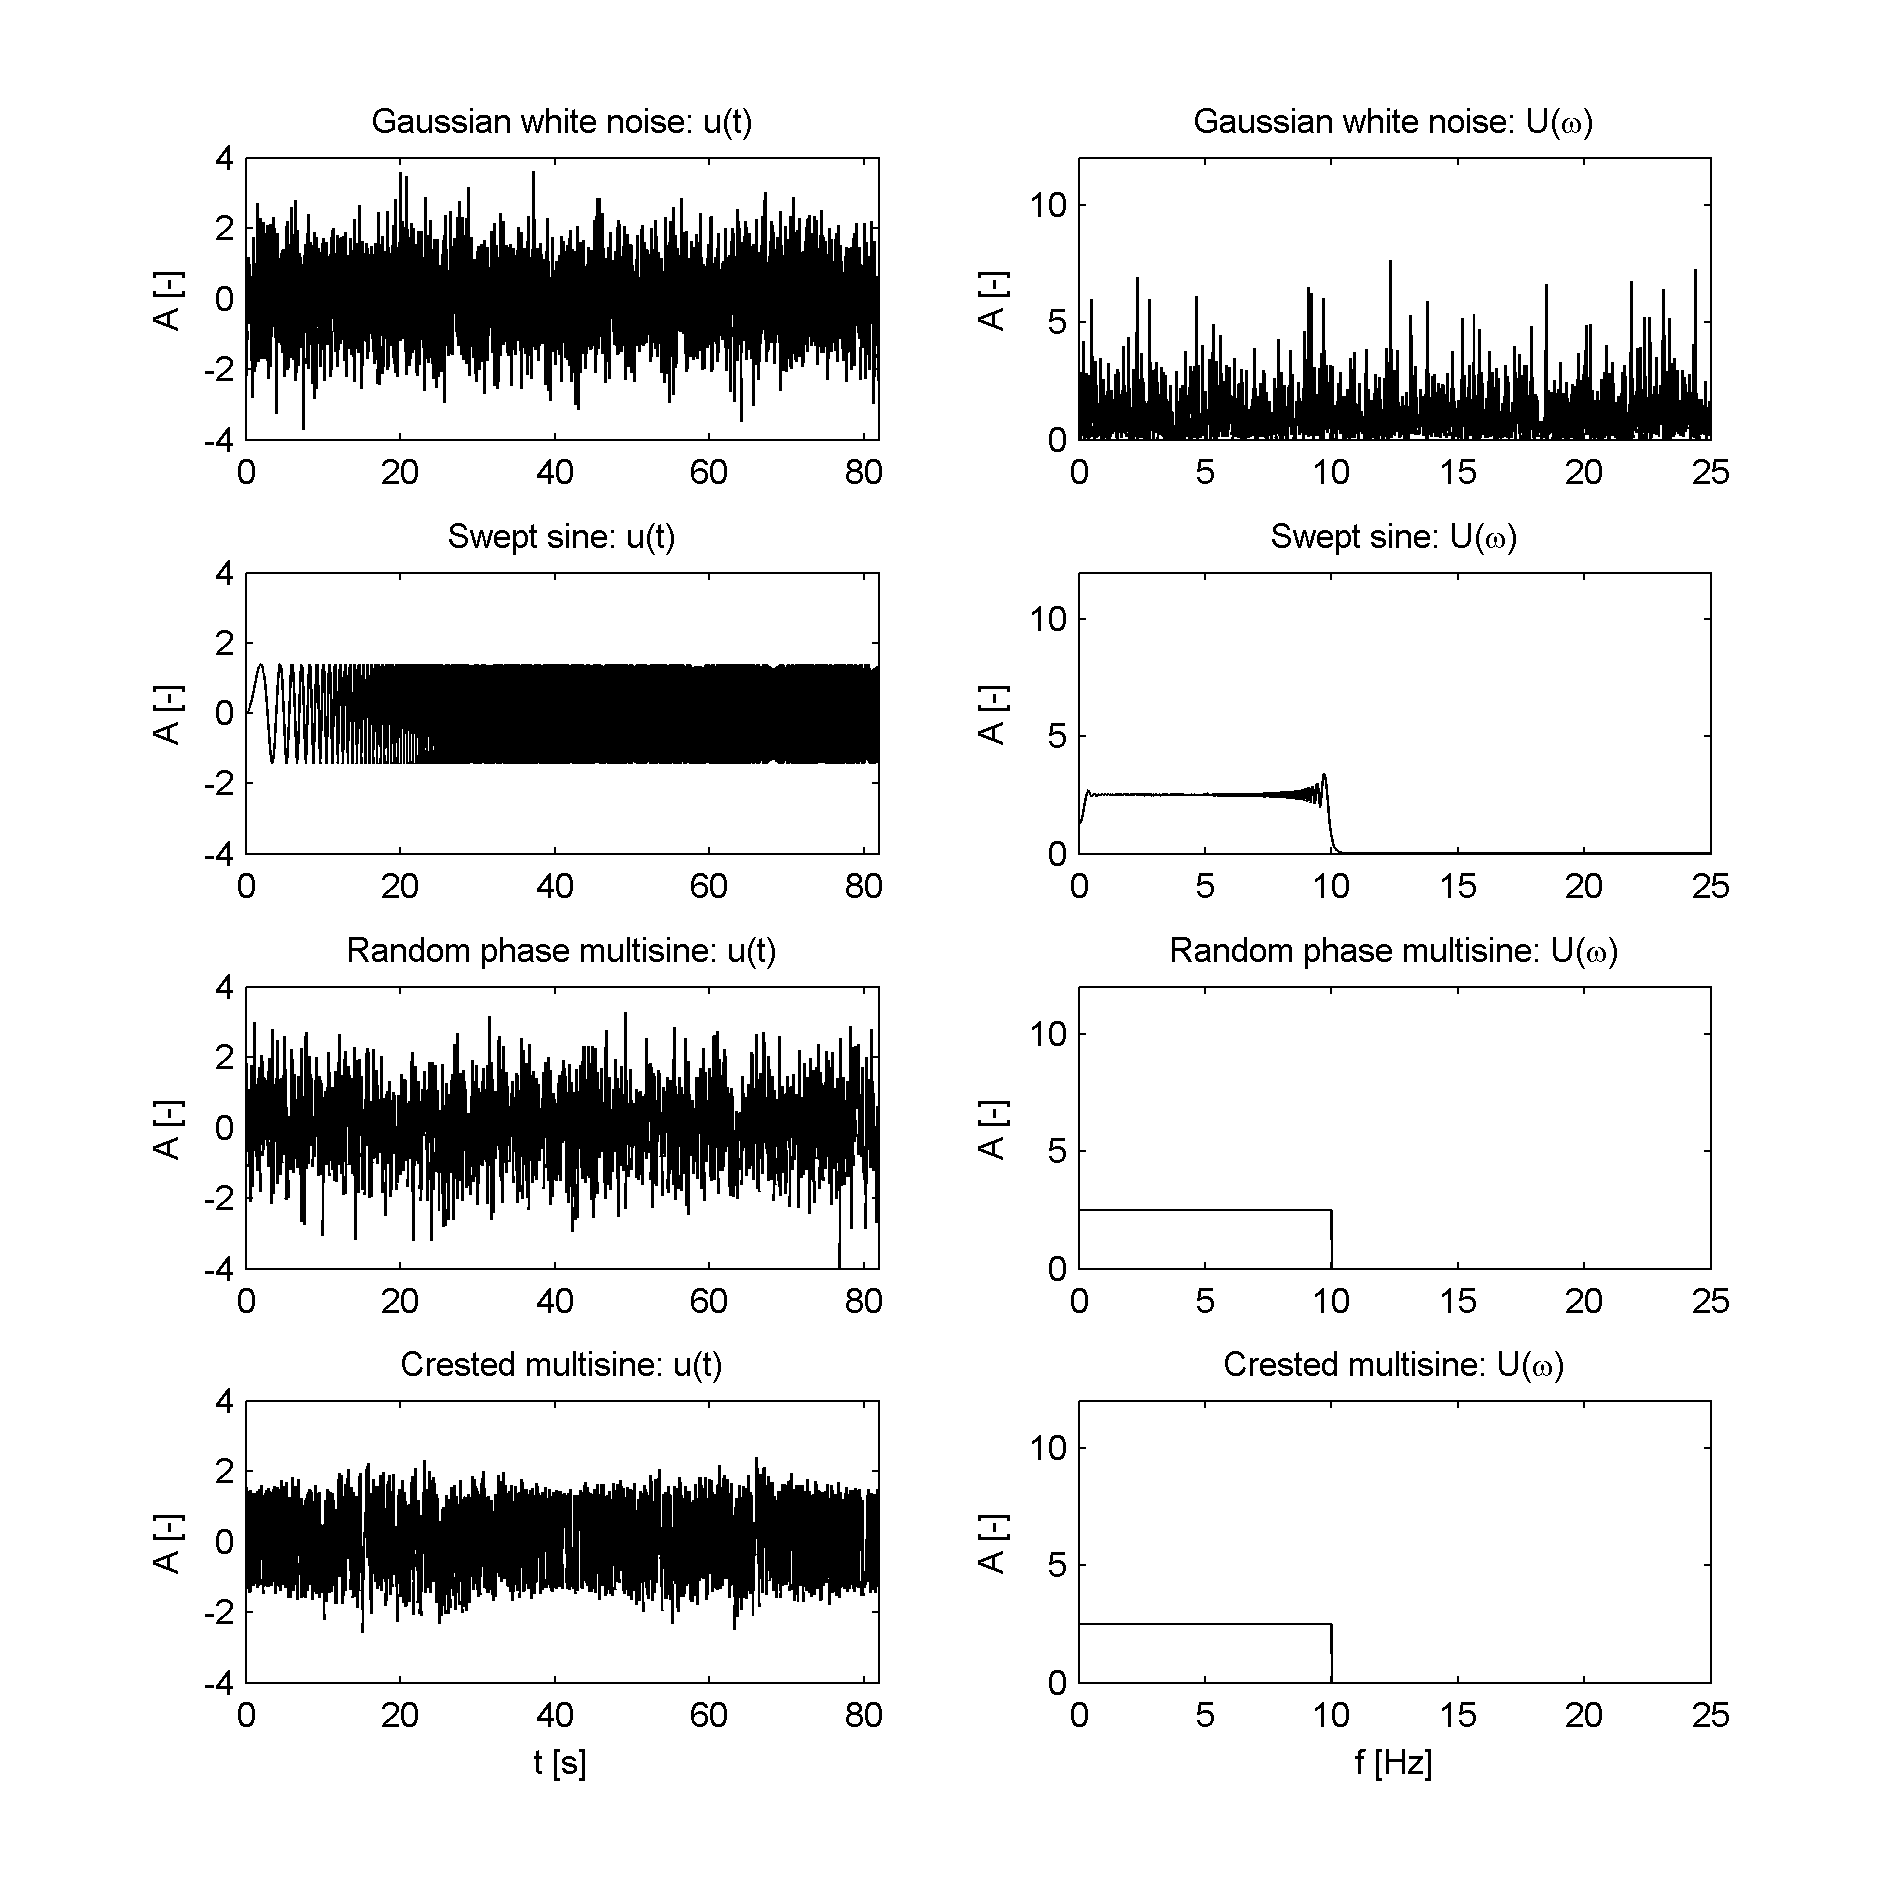
\includegraphics[scale=0.4]{images/u}
		\end{figure}
\end{frame}

\begin{frame}{Frequency averaging}
Welch method
\begin{itemize}
		\item Divide data in multiple segments
		\item Calculate spectral density for each segment
		\item Average over the segments
		\item D-time segments
		\item Drawback: reduced spectral resolution with factor D:
		\begin{equation} \hat{S}_{uy}(\omega) = \frac{1}{D}\sum^D_{d=1}S_{uy}(\omega) \end{equation}
\end{itemize}
Frequency averaging
\begin{itemize}
\item Calculate the raw spectral density
\item Average over adjacent frequencies over bandwidth D
\begin{equation} \hat{S}_{uy}(\omega_c) = \frac{1}{D}\sum^D_{d=1}\hat{S}_{uy}(\omega_d)\end{equation}
\item Drawback: Introduces bias at sharp transitions in FRF.
\end{itemize}
\end{frame}

\begin{frame}{Open loop SISO Identification}
		Considering the following SISO system $H(\omega)$ with white observation noise $n$:
		% We need layers to draw the block diagram
\begin{figure}[ht]
\centering %

\tikzstyle{block} = [draw,rectangle,thick,minimum height=2em,minimum width=2em]
\tikzstyle{bigblock} = [draw,rectangle,thick,minimum height=2em,minimum width=3em]
\tikzstyle{sum} = [draw,circle,inner sep=0mm,minimum size=2mm]
\tikzstyle{connector} = [->,thick]
\tikzstyle{line} = [thick]	

\tikzstyle{branch} = [circle,inner sep=0pt,minimum size=1mm,fill=black,draw=black]
\tikzstyle{guide} = []

\begin{tikzpicture}[scale=1, auto]

    %  Loop function
    \node[coordinate]												(input) 		{};
		\node[coordinate,right of=input]		(u)	{};
		\node[block,right of =u] 			(H) 					{$H$};
		\node[sum,right of=H]				(sumn)			{};
		\node[coordinate,above of=sumn]				(n)			{};
		\node[coordinate,right of =sumn]				(y) 					{$\mathbf{H}$};
		\node[coordinate,right of =y]				(output) 				{};
		
		% Draw connectors
		\draw[connector] (input) -- node {$u$} (H);
		\draw[connector] (H) -- node {} (sumn);
				\draw[connector] (sumn) -- node {$y$} (output);
		\draw[connector] (n) -- node {$n$} (sumn);	

    \end{tikzpicture}
		
		\end{figure}
		Solving the block diagram for the unknown system $H(\omega)$ gives:
		\begin{align}
		Hu & = y-n 
		\end{align}
		Unfortunately we cant solve for $H$, since the noise term is unknown. However, assuming the noise $n$ is uncorrelated with $u$ we can estimate the system:
				\begin{align}
						u^\ast Hu & = u^\ast (y-n) \nonumber \\
						H 					& = \frac{u^\ast (y-n)}{u^\ast u} =  \frac{\hat{S}_{uy} - \hat{S}_{un}}{\hat{S}_{uu}}  \nonumber \\
						\hat{H}	& = \frac{\hat{S}_{uy}}{\hat{S}_{uu}} \ \ \textrm{, if} \ \hat{S}_{un} \approx 0
				\end{align}
\end{frame}

\begin{frame}{SISO example}
\begin{figure}
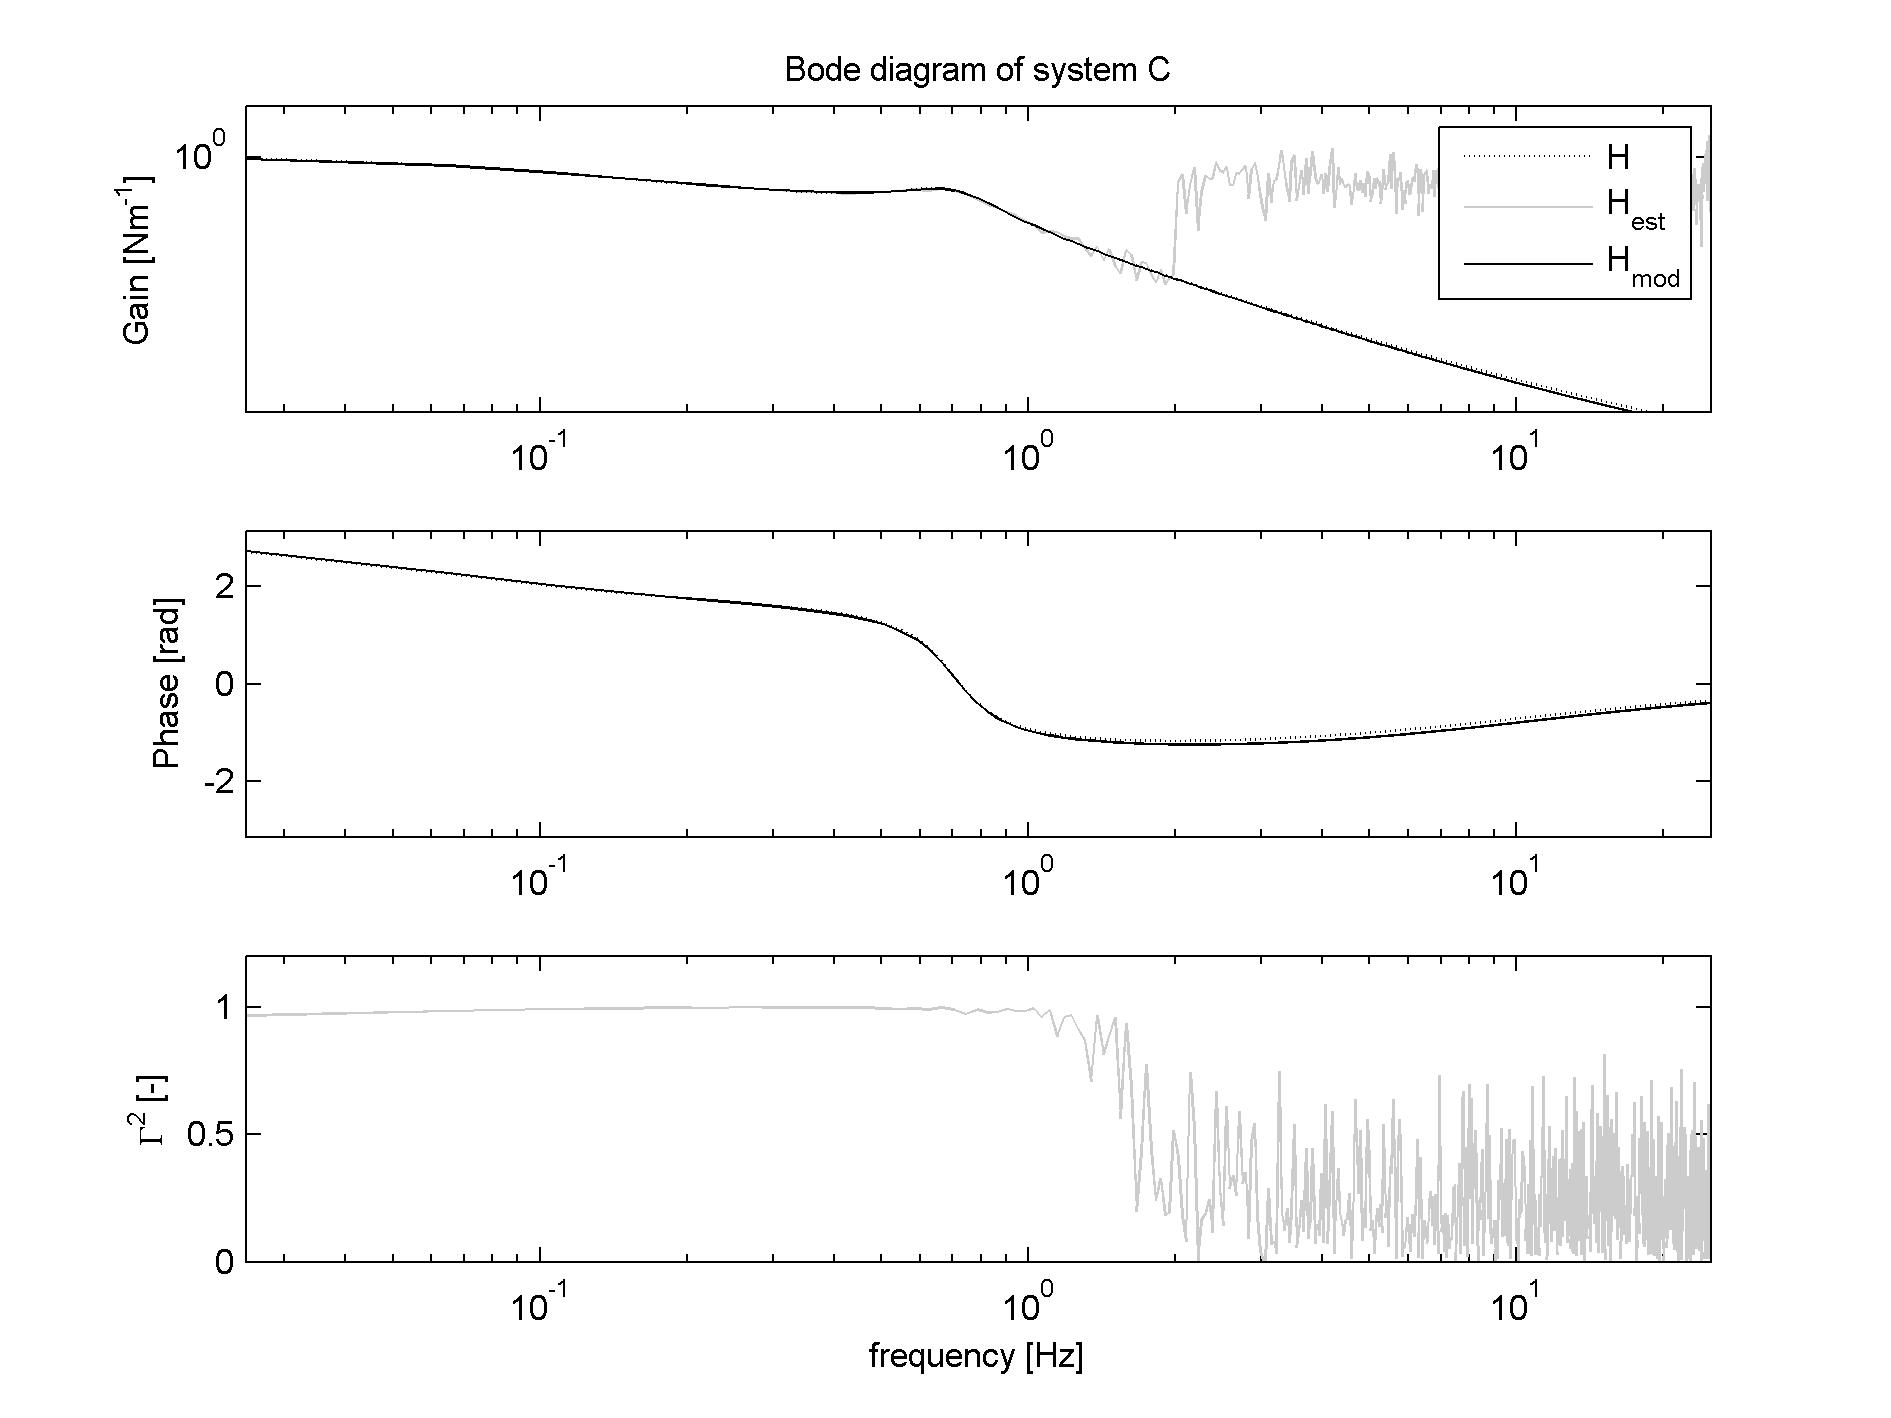
\includegraphics[scale=0.6]{images/SISObode}
\end{figure}
\end{frame}

\begin{frame}{Open loop MIMO Identification}
		Similar to the SISO case, we can use the same strategy to solve for the MIMO case:
		\begin{align}
				\mathbf{H}\mathbf{U} & = \mathbf{Y}-\mathbf{N}  \nonumber \\
				\mathbf{U}^\ast\mathbf{H}^\ast & = \mathbf{Y}^\ast-\mathbf{N} ^\ast \nonumber \\
					\mathbf{U}\mathbf{U}^\ast\mathbf{H}^\ast & = 	\mathbf{U}\left(\mathbf{Y}^*-\mathbf{N} ^\ast\right) \nonumber \\
					\mathbf{H}^\ast & = 	\left(\mathbf{U}\mathbf{U}^\ast\right)^{-1}\mathbf{U}\left(\mathbf{Y}^\ast-\mathbf{N} ^\ast\right) \nonumber \\
								\mathbf{H} & = 	\left(\mathbf{Y}-\mathbf{N}\right)\mathbf{U}^\ast\left(\mathbf{U}\mathbf{U}^\ast\right)^{-1} 
		\end{align}
Next we define the estimated transferfunction $\hat{\mathbf{H}}$ to be the transferfunction that linearly correlates the input/output data, assuming that the input is uncorrelated with the noise.
	\begin{align}
				\hat{\mathbf{H}} 	= & \mathbf{Y}\mathbf{U}^\ast\left(\mathbf{U}\mathbf{U}^\ast\right)^{-1} =  \hat{\mathbf{S}}_{yu}\hat{\mathbf{S}}_{uu}^{-1}
	\end{align}
\end{frame}

\begin{frame}{MIMO example}
\begin{figure}
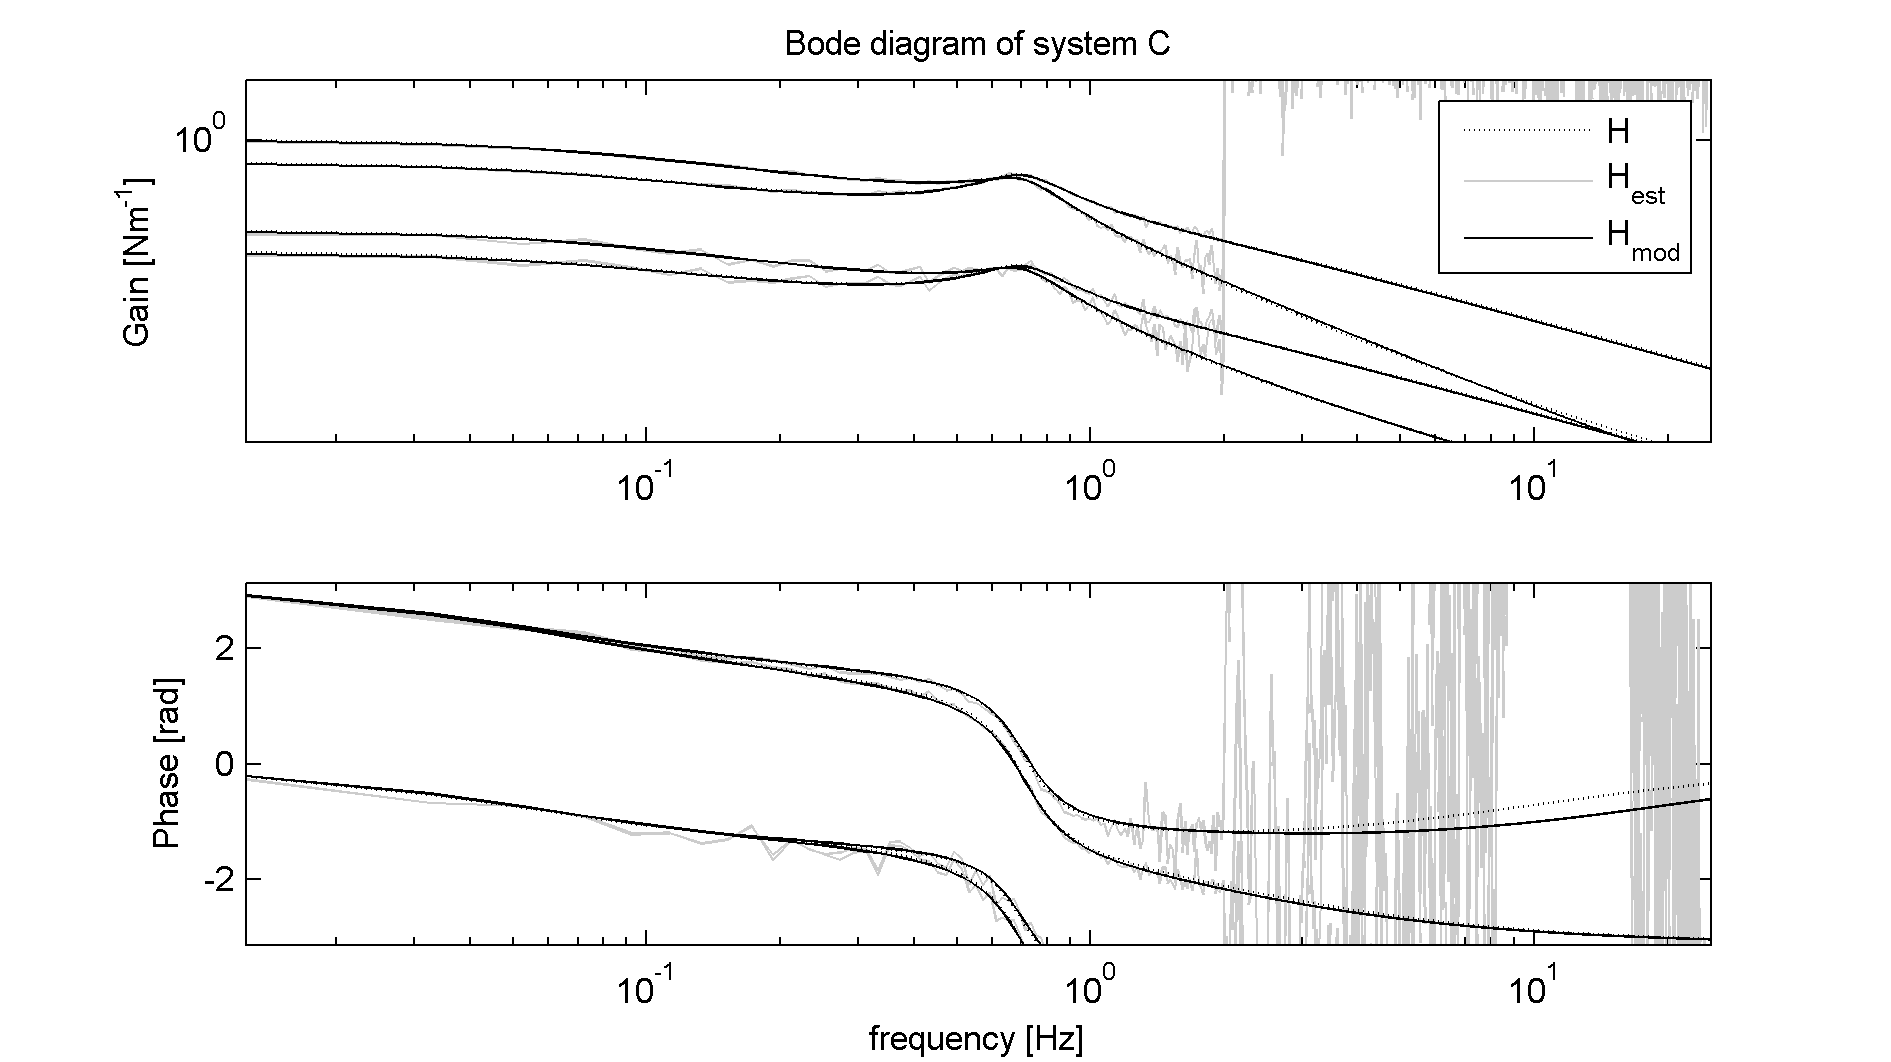
\includegraphics[scale=0.6]{images/MIMObode}
\end{figure}
\end{frame}

\begin{frame}{Close loop identification}
Suppose we have a closed loop system shown in the block diagram below:
% We need layers to draw the block diagram
\begin{figure}[ht]
\centering %

\tikzstyle{block} = [draw,rectangle,thick,minimum height=2em,minimum width=2em]
\tikzstyle{bigblock} = [draw,rectangle,thick,minimum height=2em,minimum width=3em]
\tikzstyle{sum} = [draw,circle,inner sep=0mm,minimum size=2mm]
\tikzstyle{connector} = [->,thick]
\tikzstyle{line} = [thick]	

\tikzstyle{branch} = [circle,inner sep=0pt,minimum size=1mm,fill=black,draw=black]
\tikzstyle{guide} = []

\begin{tikzpicture}[scale=1, auto]

    %  Loop function
    \node[coordinate]												(input) 		{};
		\node[sum,right of=input]		(u)	{};
		\node[block,right of =u] 			(H) 					{$H$};
		\node[sum,right of=H]				(sumn)			{};
		\node[coordinate,above of=sumn]				(n)			{};
		\node[coordinate,right of =sumn]				(y) 					{$\mathbf{H}$};
		\node[coordinate,right of =y]				(output) 				{};
		
		\node[coordinate,below of = y] (yfb) {};
		\node[coordinate,below of = u] (sumu) {};
		
		% Draw connectors
		\draw[connector] (input) -- node {$r$} (u);
				\draw[connector] (u) -- node {$u$} (H);
		\draw[connector] (H) -- node {} (sumn);
				\draw[connector] (sumn) -- node {$y$} (output);
		\draw[connector] (n) -- node {$n$} (sumn);	
		
		\draw[connector] (y) -- (yfb) -- (sumu) -- (u);

    \end{tikzpicture}
		
		\end{figure}
Than the open loop estimator $\hat{H}=S_{uy}/S_{uu}$ no longer holds, because the noise is correlated with the input signal through the feedback loop:
\begin{equation} 						\hat{H}	\neq \frac{S_{uy}}{S_{uu}} \end{equation}
\end{frame}

\begin{frame}{Not discussed}
		\begin{itemize}
		\item Windowing  techniques: prevents or reduces spectral leaking.
		\item MIMO coherence: seperating coherent inputs/outputs.
		\item Closed loop system estimation
		\item Parameter Estimation in the frequency domain
		\end{itemize}
\end{frame}

\begin{frame}{Conclusions}
	\begin{itemize}
	\item Frequency domain estimation techniques are well suited for linear dynamic deterministic systems.
	\item Proper input signal design can boost the signal to noise ratio.
	\item Frequency averaging should be applied to average out the noise.
	\item Don't use openloop SISO estimator when feedback is present in the system!
	\end{itemize}
\end{frame}

\begin{frame}{Further information}
Some references about system identification and parameter estimation.
		\begin{itemize}
		\item System Identification: A frequency domain approach - Pintelon and Schoukens 
		\item Filtering and Identification - Verhaegen and Verdult
		\end{itemize}
\end{frame}


\end{document}
